\section{Анализ предметной области}

\subsection{Обзор аналогов}

Веб-сайт eBay - это международная онлайн-аукционная платформа, 
которая позволяет пользователям покупать и продавать товары. 
eBay была основана в 1995 году и является одним из крупнейших онлайн-аукционов в мире.

Система eBay предлагает широкий спектр функций.
В частности данная платформа позволяет пользователям создавать аукционы на различные товары, 
включая антиквариат, коллекционные предметы, электронные устройства и многое другое. 
Пользователи могут делать ставки на товары, а также покупать товары в режиме реального времени.

Кроме того, eBay Seller Center предоставляет широкие возможности для интеграции 
с внешними системами и сервисами. 
% Развитые API-интерфейсы позволяют 
% легко связывать серверное приложение аукциона с другими бизнес-приложениями, 
% такими как CRM, ERP или складской учет. 
Это дает продавцам возможность автоматизировать многие рутинные операции и повысить эффективность своей работы на eBay.
Скриншот веб-сайта «eBay» указан на рисунке 1.1.

\begin{figure}[ht]
\centering
    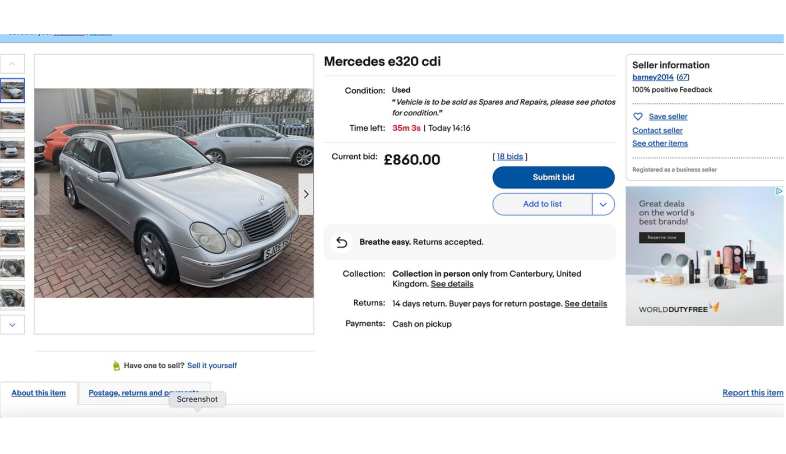
\includegraphics[scale=0.5]{ebay.png}
    \caption{Скриншот веб-сайта «eBay»}
\end{figure}

Auction House Management System (AHMS) - это комплексное сервер-
ное приложение, предназначенное для управления деятельностью професси-
ональных аукционных домов. Оно охватывает весь цикл аукционного процес-
са: от каталогизации лотов и регистрации участников до проведения торгов,
осуществления расчетов и формирования всесторонней отчетности.
Также данная система может предоставить полную историю торгов.
Скриншот проведения аукционов в системе AHMS показан на рисунке 1.2.


\begin{figure}[h]
\centering
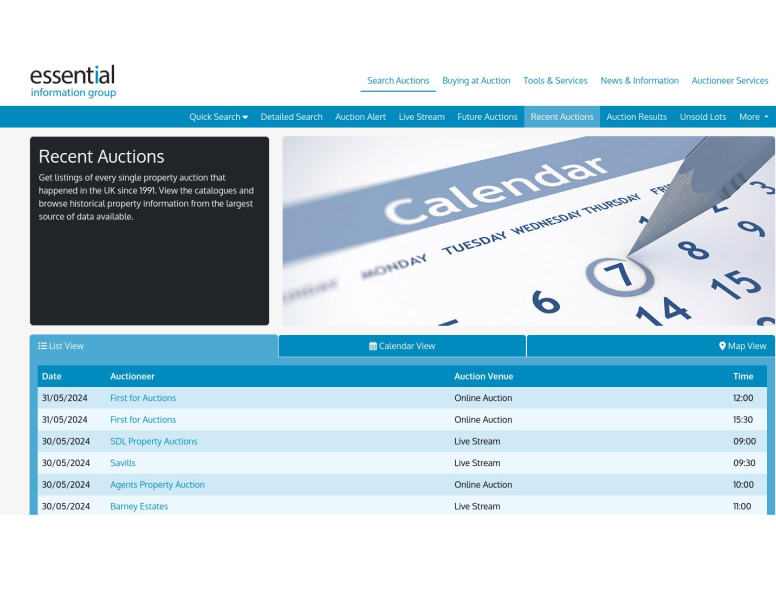
\includegraphics[scale=0.3]{ahms.png}
\caption{Скриншот системы «Auction House Management System»}
\end{figure}
Анализ данных средств, позволяет выявить функциональные требования к нашей системе.

% Одной из ключевых особенностей AHMS является его высокая гибкость и возможность адаптации под конкретные требования 
% и бизнес-процессы каждого аукционного дома. 
% Платформа предоставляет широкие возможности для настройки интерфейсов, workflows, 
% правил и алгоритмов работы. Это позволяет аукционным домам внедрять AHMS, 
% не меняя сложившиеся практики ведения бизнеса, а лишь адаптируя приложение под свои нужды.

\subsection{Постановка задачи}

В рамках данного курсового проекта была поставлена задача:
разработать серверную часть системы управления аукционом.

Был выделен
следующий ряд подзадач:

– описать модели данных проекта, включая модели для лотов, категорий лотов, ставок, пользователей;

– реализовать механизмы сохранения, чтения, обновления и удаления
данных в инструментах хранения данных;

– реализовать функционал создания аукциона, создание ставок;

– реализовать механизмы авторизации и аутентификации по ролям;

– реализовать механизмы администрирования системы аукциона;

– разработать приложение в формате веб-приложения;

– реализовать механизмы уведомления пользователей об изменном состоянии аукциона в режиме реального времени;

– разработать интерактивную документацию, которая будет содержать
подробное описание функциональности системы, API-интерфейсов.

Разработав данный набор задач можно перейти непосредственно к
проектированию программного средства.